\subsection{Eigendecomposition ($A = P DP ^{-1}$)}

\begin{figure}[H]
    \centering
    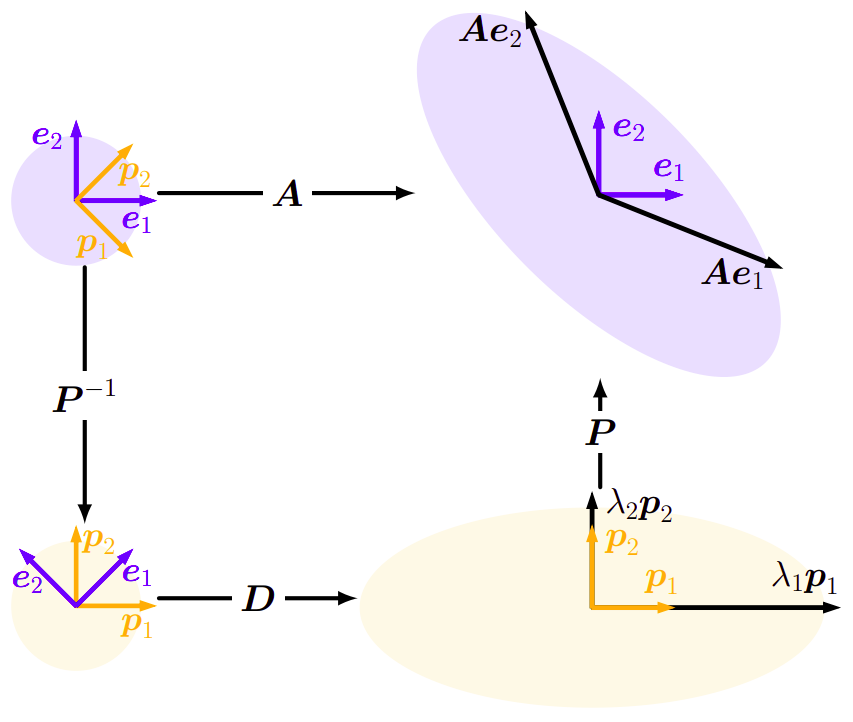
\includegraphics[
        width=\linewidth,
        height=5cm,
        keepaspectratio,
    ]{images/maths-for-ml/eigendecomposition.png}
    \caption*{
        Intuition behind the eigendecomposition as sequential transformations.
        \\
        \textbf{Top-left to bottom-left}: $\bm{P}^{-1}$ performs a basis change (here drawn in $\mathbb{R}^2$ and depicted as a rotation-like operation) from the standard basis into the eigenbasis.
        \\
        \textbf{Bottom-left to bottom-right}: $\bm{D}$ performs a scaling along the remapped orthogonal eigenvectors, depicted here by a circle being stretched to an ellipse. 
        \\
        \textbf{Bottom-right to top-right}: $\bm{P}$ undoes the basis change (depicted as a reverse rotation) and restores the original coordinate frame.
    }
\end{figure}


\begin{enumerate}
    \item 
    \begin{theorem}[Eigendecomposition]
        A square matrix $\bm{A} \in \mathbb{R}^{n\times n}$ can be factored into $\bm{A} = \bm{PDP}^{-1}$ where $\bm{P} \in \mathbb{R}^{n\times n}$ and $\bm{D}$ is a diagonal matrix whose diagonal entries are the eigenvalues of $\bm{A}$, if and only if the eigenvectors of $\bm{A}$ form a basis of $\mathbb{R}^n$.
        \hfill \cite{mfml/book/mml/Deisenroth-Faisal-Ong}
    \end{theorem}

    \item \textbf{Steps}:
    \begin{enumerate}
        \item Compute eigenvalues and eigenvectors

        \item Check for existence (eigenvectors span $\mathbb{R}^n$ or not)

        \item Construct the matrix P to diagonalize A
        \begin{enumerate}
            \item $\bm{P} = [\bm{p}_1, \cdots, \bm{p}_n]$

            \item $\bm{D} = \bm{P}^{-1}\bm{AP} = \bm{P}^{\top}\bm{AP}$
        \end{enumerate}
    \end{enumerate}

    \item we can find a matrix power for a matrix $\bm{A} \in \mathbb{R}^{n\times n}$ via the eigenvalue decomposition (if it exists) so that:
    \hfill \cite{mfml/book/mml/Deisenroth-Faisal-Ong}
    \\
    .\hfill
    $
        \bm{A}^k 
        = (\bm{PDP}^{-1})^k 
        = \bm{PDP}^{-1}\bm{PDP}^{-1}\cdots \bm{PDP}^{-1} 
        = \bm{PD}^k \bm{P}^{-1}
    $
    \hfill \cite{mfml/book/mml/Deisenroth-Faisal-Ong}

    \item Assume that the eigendecomposition $\bm{A} = (\bm{PDP}^{-1})$ exists. Then: 
    \hfill \cite{mfml/book/mml/Deisenroth-Faisal-Ong}
    \\
    .\hfill
    $
        \det(\bm{A}) 
        = \det(\bm{PDP}^{ -1}) 
        = \det(\bm{P}) \det(\bm{D}) \det(\bm{P}^{-1})
        = \det(\bm{D})
        = \dprod_{i} d_{ii}
    $
    \hfill \cite{mfml/book/mml/Deisenroth-Faisal-Ong}
\end{enumerate}



\begin{lstlisting}[
    language=Python,
    caption=Eigendecomposition - numPy
]
import numpy as np

# Define a square matrix
A = np.array([[4, -2],
              [1,  1]])

# Perform eigendecomposition
eigenvalues, eigenvectors = np.linalg.eig(A)

# Construct D and P
D = np.diag(eigenvalues)
P = eigenvectors

# Inverse of P
P_inv = np.linalg.inv(P)

# Reconstruct A
A_reconstructed = P @ D @ P_inv

# Print results
print("Original matrix A:")
print(A)

print("\nEigenvalues (D):")
print(D)

print("\nEigenvectors (P):")
print(P)

print("\nReconstructed A (P D P_inv):")
print(A_reconstructed)

print("\nCheck reconstruction accuracy:", np.allclose(A, A_reconstructed))
\end{lstlisting}






